\documentclass[tikz,border=0pt]{standalone}
\usepackage[american]{circuitikz}
\usetikzlibrary{arrows.meta,calc,positioning,decorations.pathmorphing,patterns}
\definecolor{zyloTeal}{HTML}{174A5B}
\definecolor{zyloTealTwo}{HTML}{246B7A}
\definecolor{zyloInk}{HTML}{1F2933}
\definecolor{zyloSoft}{HTML}{EAF4F4}
\definecolor{zyloPaper}{HTML}{F8FAFB}
\definecolor{zyloLine}{HTML}{44606B}
\definecolor{zyloOrange}{HTML}{D97706}
\begin{document}
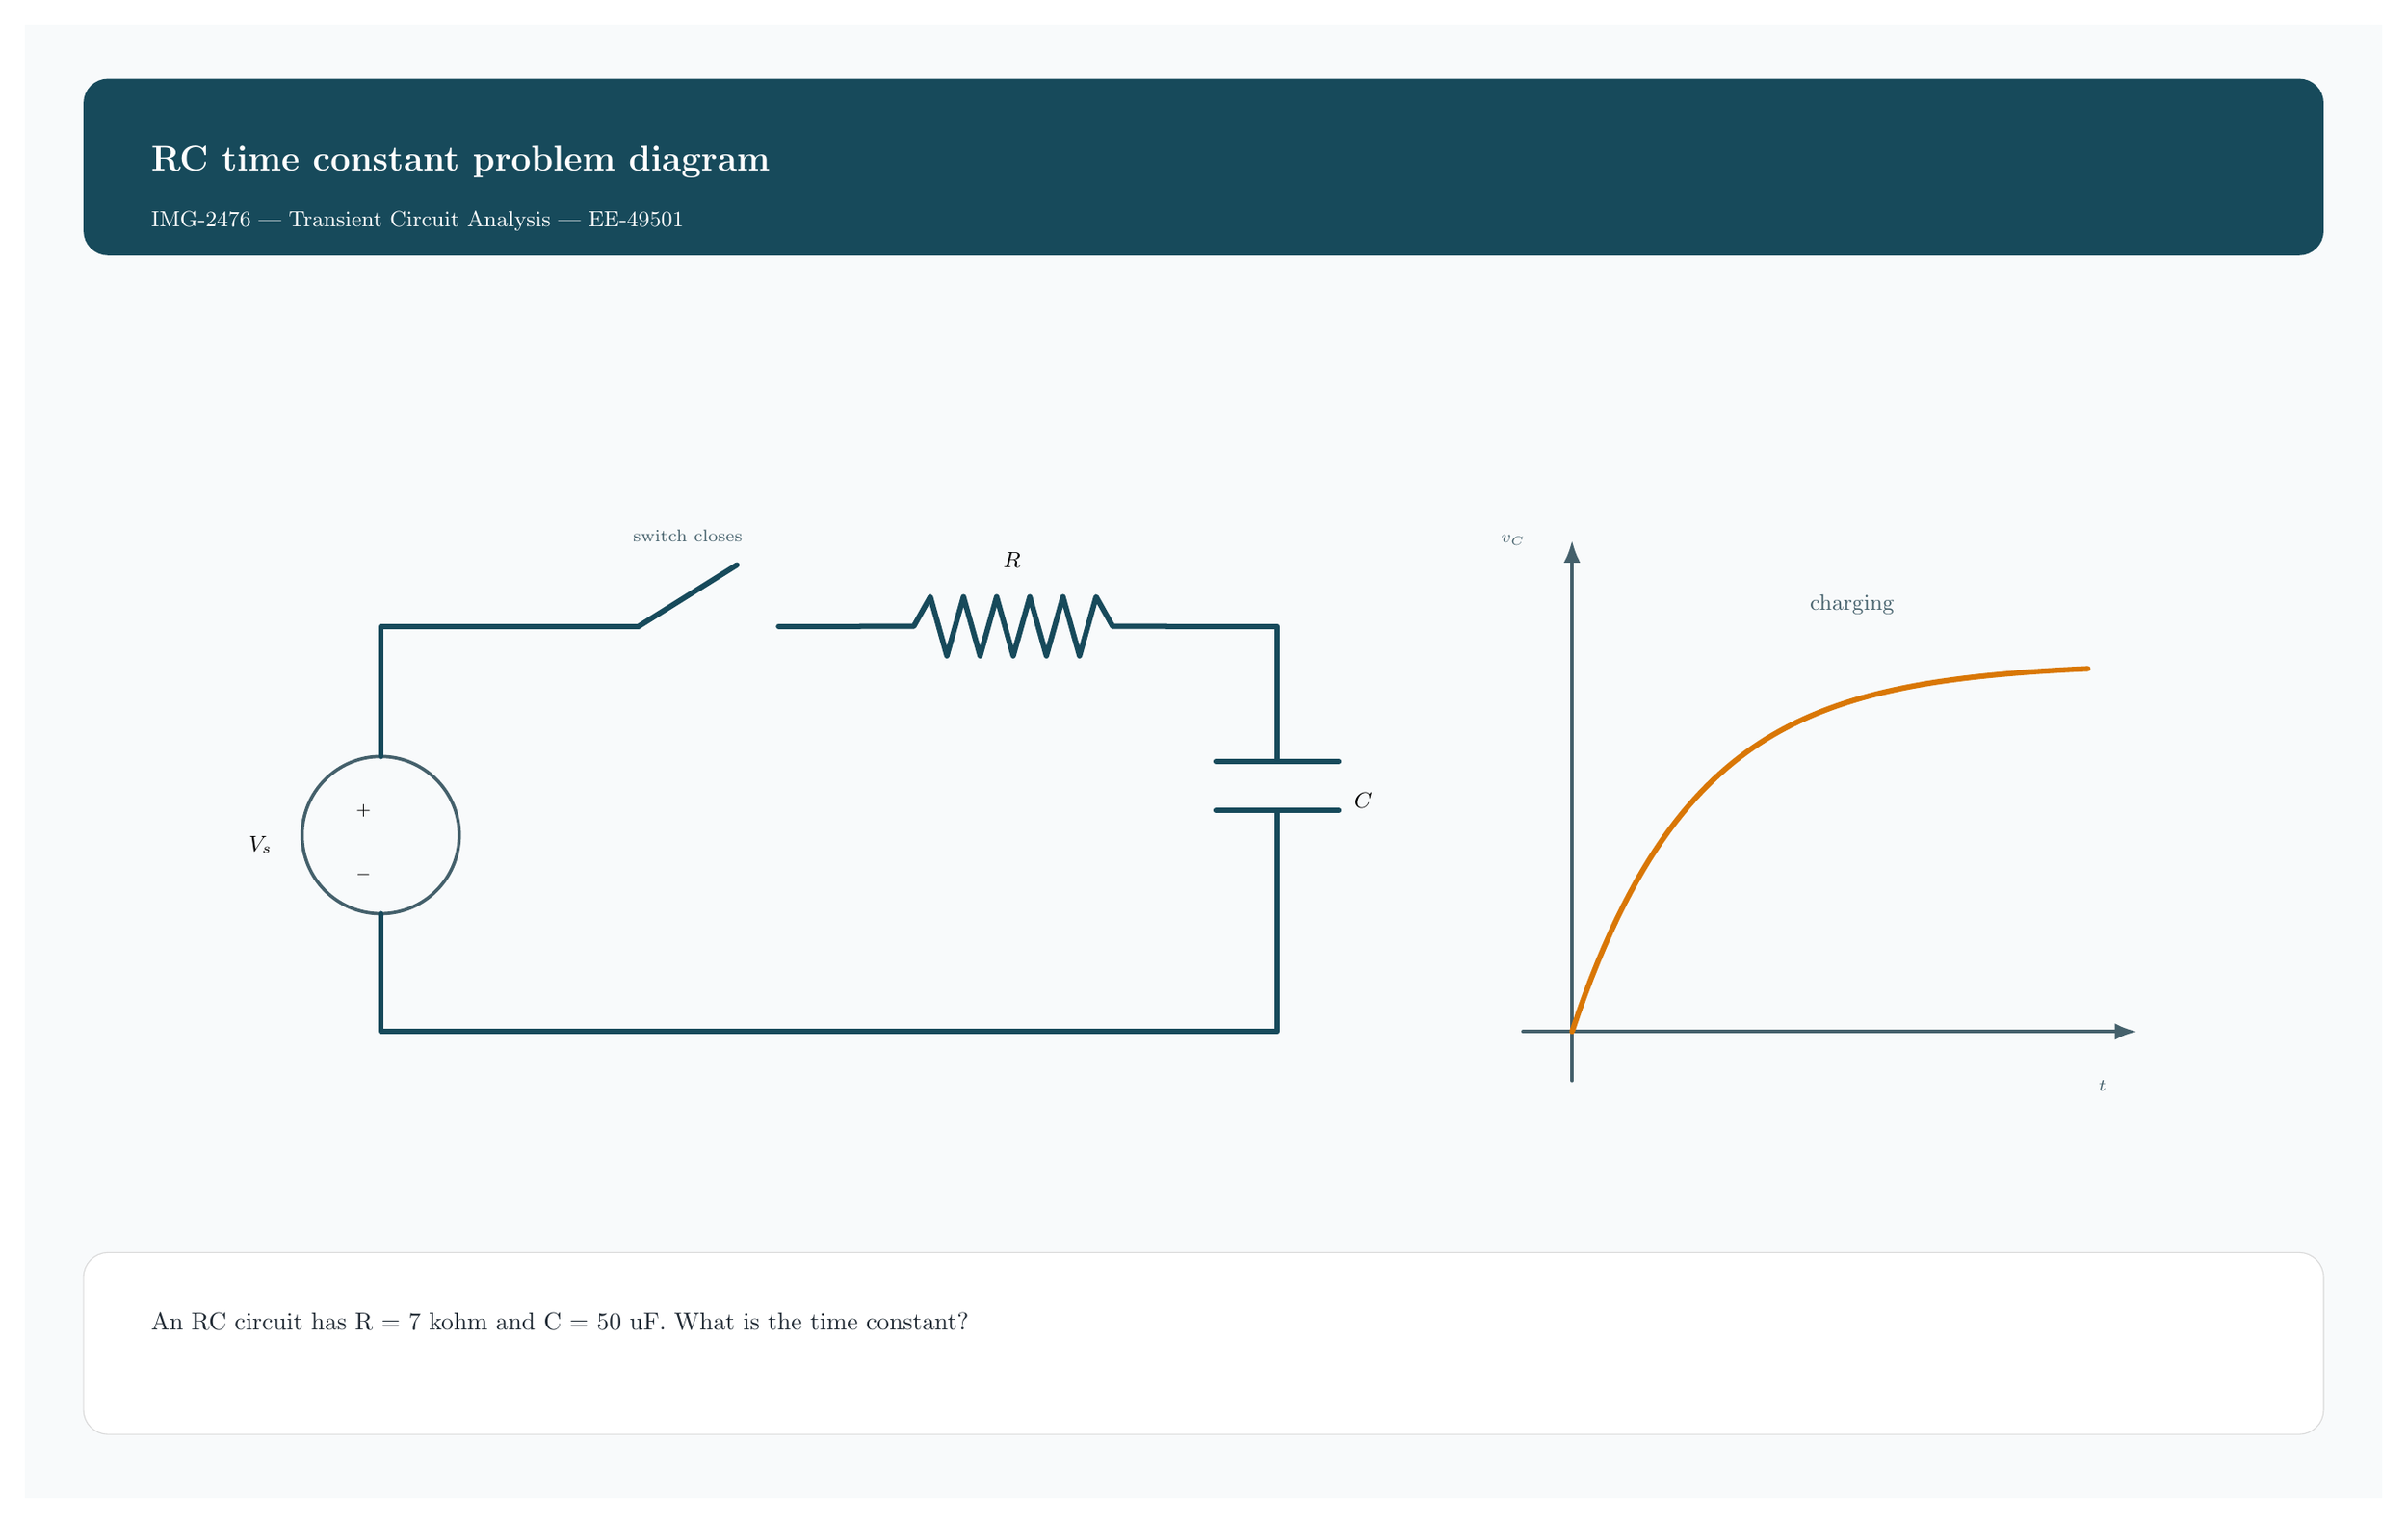
\begin{tikzpicture}[x=1pt,y=-1pt,>=Latex,line cap=round,line join=round]
\path[fill=zyloPaper] (0,0) rectangle (960,600);
\path[fill=zyloTeal,rounded corners=10pt] (24,22) rectangle (936,94);
\node[anchor=west,text=white,font=\bfseries\Large] at (48,56) {RC time constant problem diagram};
\node[anchor=west,text=white!82,font=\small] at (48,80) {IMG-2476 | Transient Circuit Analysis | EE-49501};
\tikzset{wire/.style={draw=zyloTeal,line width=2.2pt},thinwire/.style={draw=zyloLine,line width=1.35pt},accent/.style={draw=zyloOrange,line width=2.2pt},box/.style={draw=zyloTealTwo,fill=zyloSoft,line width=1.5pt,rounded corners=8pt}}
\draw[thinwire] (145,330) circle (32); \node[font=\scriptsize] at (138,320) {$+$}; \node[font=\scriptsize] at (138,346) {$-$}; \node[font=\small] at (96,334) {$V_s$};
\draw[wire] (145,298) -- (145,245) -- (250,245); \draw[wire] (250,245) -- (290,220); \draw[wire] (307,245) -- (340,245);
\draw[wire] (340,245) -- (362,245) -- (362,245) -- (368.75,233) -- (375.5,257) -- (382.25,233) -- (389,257) -- (395.75,233) -- (402.5,257) -- (409.25,233) -- (416,257) -- (422.75,233) -- (429.5,257) -- (436.25,233) -- (443,245) -- (465,245);
\draw[wire] (465,245) -- (510,245) -- (510,300); \draw[wire] (485,300) -- (535,300); \draw[wire] (485,320) -- (535,320); \draw[wire] (510,320) -- (510,410) -- (145,410) -- (145,362);
\node[font=\small] at (402,218) {$R$}; \node[font=\small] at (545,316) {$C$}; \node[font=\scriptsize,text=zyloLine] at (270,208) {switch closes};
\draw[thinwire,->] (610,410) -- (860,410); \draw[thinwire,->] (630,430) -- (630,210);
\draw[accent] (630,410) -- (632.625,402.328) -- (635.25,395.049) -- (637.875,388.142) -- (640.5,381.588) -- (643.125,375.369) -- (645.75,369.468) -- (648.375,363.869) -- (651,358.557) -- (653.625,353.516) -- (656.25,348.733) -- (658.875,344.195) -- (661.5,339.889) -- (664.125,335.803) -- (666.75,331.926) -- (669.375,328.247) -- (672,324.757) -- (674.625,321.445) -- (677.25,318.302) -- (679.875,315.32) -- (682.5,312.491) -- (685.125,309.806) -- (687.75,307.259) -- (690.375,304.842) -- (693,302.548) -- (695.625,300.372) -- (698.25,298.307) -- (700.875,296.348) -- (703.5,294.489) -- (706.125,292.725) -- (708.75,291.051) -- (711.375,289.463) -- (714,287.956) -- (716.625,286.526) -- (719.25,285.17) -- (721.875,283.882) -- (724.5,282.661) -- (727.125,281.502) -- (729.75,280.402) -- (732.375,279.359) -- (735,278.368) -- (737.625,277.429) -- (740.25,276.538) -- (742.875,275.692) -- (745.5,274.889) -- (748.125,274.128) -- (750.75,273.405) -- (753.375,272.719) -- (756,272.069) -- (758.625,271.452) -- (761.25,270.866) -- (763.875,270.31) -- (766.5,269.783) -- (769.125,269.283) -- (771.75,268.808) -- (774.375,268.357) -- (777,267.93) -- (779.625,267.524) -- (782.25,267.139) -- (784.875,266.774) -- (787.5,266.428) -- (790.125,266.099) -- (792.75,265.787) -- (795.375,265.491) -- (798,265.21) -- (800.625,264.944) -- (803.25,264.691) -- (805.875,264.451) -- (808.5,264.223) -- (811.125,264.007) -- (813.75,263.802) -- (816.375,263.608) -- (819,263.423) -- (821.625,263.248) -- (824.25,263.082) -- (826.875,262.925) -- (829.5,262.775) -- (832.125,262.633) -- (834.75,262.498) -- (837.375,262.371) -- (840,262.249);
\node[font=\scriptsize,text=zyloLine] at (846,432) {$t$}; \node[font=\scriptsize,text=zyloLine] at (606,210) {$v_C$}; \node[font=\small,text=zyloLine] at (744,236) {charging};
\path[draw=black!15,fill=white,rounded corners=10pt] (24,500) rectangle (936,574);
\node[anchor=west,text width=860pt,align=left,text=zyloInk,font=\normalsize] at (48,528) {An RC circuit has R = 7 kohm and C = 50 uF. What is the time constant?};
\end{tikzpicture}
\end{document}
